\documentclass[11pt]{amsart}

\renewcommand{\baselinestretch}{1.08}

\usepackage{geometry}
\geometry{letterpaper, margin=1in}

\usepackage{verbatim,xspace,amssymb}

\usepackage{tikz}
\usetikzlibrary{arrows}

% hyperref should be the last package we load
\usepackage[pdftex,
            colorlinks=true,
            plainpages=false,
            linkcolor=blue,   % only if colorlinks=true
            citecolor=red,    % only if colorlinks=true
            urlcolor=magenta  % only if colorlinks=true
]{hyperref}

% math macros
\newcommand\bb{\mathbf{b}}
\newcommand\bbf{\mathbf{f}}
\newcommand\bn{\mathbf{n}}
\newcommand\bq{\mathbf{q}}
\newcommand\bu{\mathbf{u}}
\newcommand\bv{\mathbf{v}}
\newcommand\by{\mathbf{y}}

\newcommand\bQ{\mathbf{Q}}
\newcommand\bV{\mathbf{V}}
\newcommand\bX{\mathbf{X}}

\newcommand\CC{\mathbb{C}}
\newcommand{\DDt}[1]{\ensuremath{\frac{d #1}{d t}}}
\newcommand{\ddt}[1]{\ensuremath{\frac{\partial #1}{\partial t}}}
\newcommand{\ddx}[1]{\ensuremath{\frac{\partial #1}{\partial x}}}
\newcommand{\ddy}[1]{\ensuremath{\frac{\partial #1}{\partial y}}}
\newcommand{\ddxp}[1]{\ensuremath{\frac{\partial #1}{\partial x'}}}
\newcommand{\ddz}[1]{\ensuremath{\frac{\partial #1}{\partial z}}}
\newcommand{\ddxx}[1]{\ensuremath{\frac{\partial^2 #1}{\partial x^2}}}
\newcommand{\ddyy}[1]{\ensuremath{\frac{\partial^2 #1}{\partial y^2}}}
\newcommand{\ddxy}[1]{\ensuremath{\frac{\partial^2 #1}{\partial x \partial y}}}
\newcommand{\ddzz}[1]{\ensuremath{\frac{\partial^2 #1}{\partial z^2}}}
\newcommand{\Div}{\nabla\cdot}
\newcommand\eps{\epsilon}
\newcommand{\grad}{\nabla}
\newcommand{\ihat}{\mathbf{i}}
\newcommand{\ip}[2]{\ensuremath{\left<#1,#2\right>}}
\newcommand{\jhat}{\mathbf{j}}
\newcommand{\khat}{\mathbf{k}}
\newcommand{\nhat}{\mathbf{n}}
\newcommand\lam{\lambda}
\newcommand\lap{\triangle}
\newcommand\Matlab{\textsc{Matlab}\xspace}
\newcommand\RR{\mathbb{R}}
\newcommand\vf{\varphi}

\newcommand{\Mstar}{$\text{Mahaffy}^{\bigstar}$\xspace}

\newcommand\alpharight{\alpha_{{}_{\blacktriangleright}}}
\newcommand\alphaup{\alpha_{{\!}_{\blacktriangle}}}

\newcommand{\dxtwo}{\tfrac{\Delta x}{2}}
\newcommand{\dytwo}{\tfrac{\Delta y}{2}}



\title[The Mahaffy scheme is an FVE method]{The Mahaffy (1976) numerical scheme \\ for the shallow ice approximation \\ is a finite volume element method}

\author{Ed Bueler}


\begin{document}

%\begin{abstract}
%\end{abstract}

\maketitle

\thispagestyle{empty}


\section{Introduction} \label{sec:intro}


The finite difference (FD) scheme introduced by \cite{Mahaffy1976} for modeling the Barnes Ice Cap was used in the first clear success in modeling ice sheet flow and geometry evolution in two horizontal dimensions.  This scheme is still a widely-used choice for numerically solving the shallow ice approximation, and its accuracy properties are relatively-well understood \cite{Bueleretal2005}.   The scheme computes the ice flux at staggered-grid points using particular choices when evaluating the ice surface slope and thickness.  In a test where an analytical solution is known and the ice rheology is realistic, these choices imply higher accuracy than an alternative widely-used scheme, while using a smaller stencil (``computational molecule''), thereby reducing memory usage in implicit implementations \cite{HindmarshPayne1996}.  As a scheme for non-sliding glacier flow, it is used as part of the stress balance solution method in a membrane-stress-resolving hybrid ice dynamics model \cite{BuelerBrown2009}.

We show that in the structured grid case the Mahaffy scheme is a reasonable, though not standard, quadrature choice for a conforming Petrov-Galerkin finite element (FE) method \cite{Elmanetal2005}.  The trial functions are piecewise-bilinear on a structured grid of rectangles---i.e.~$Q^1$ finite elements \cite{Elmanetal2005}.  The test functions are piecewise-constant with support on dual rectangular control volumes, so the scheme can also be interpreted as a ``finite volume element'' (FVE) method \cite{EwingLinLin2002}.

Based on this re-interpretation of the scheme we propose, and test, a ``\Mstar'' scheme which uses a more accurate quadrature choice when evaluating the relevant flux integral, but which is based on the same stencil.  Furthermore, we construct this \Mstar scheme on unstructured grids consisting of suitable finite element triangulations with dual control volumes, i.e.~Delaunay/Voronoi dual meshes (compare \cite{Ringleretal2013}).

MAYBE NOT: The accuracy of the Mahaffy scheme on steep bed terrain has been found to be flawed, but corrections have been proposed \cite{JaroschSchoofAnslow2013}.  We show that these corrections are unnecessary in the \Mstar scheme.


\section{The Mahaffy finite difference scheme}   \label{sec:mahaffyfd}

The shallow ice approximation (SIA) \cite{Hutter1983} is the lubrication approximation \cite{Fowler1997} of the Stokes equations for slow-flowing ice which is in non-sliding contact with the bed and which has a freely-evolving upper surface.  We only consider the isothermal, Glen-power-law (e.g.~\cite{GreveBlatter2009}) case of the shallow ice approximation.

Let $H$ be the ice thickness, $b$ the bed elevation, and $s = H+b$ the ice surface elevation.  The ice sheet thickness evolution itself is a straightforward conservation equation,
\begin{equation}
\frac{\partial H}{\partial t} + \Div \bq = m  \label{eq:siaevolution}
\end{equation}
where $m$ [SI units $\text{m}/\text{s}$] is the surface mass balance, also called the accumulation/ablation function, and the divergence ``$\Div$'' is computed in horizontal $x,y$ directions only.  In the SIA the vertically-integrated flux [units $\text{m}^2/\text{s}$], or volume flux \cite{GreveBlatter2009}, is
\begin{equation}
\bq = - \Gamma H^{n+2} |\grad s|^{n-1} \grad s  \label{eq:siaflux}
\end{equation}
where $\Gamma = 2 A (\rho g)^n / (n+2)$ is a positive constant, in the isothermal case, and ``$\grad$'' is the gradient in $x,y$.

The flux \eqref{eq:siaflux} has a couple of interpretations in the literature.  Equation \eqref{eq:siaevolution} can be interpreted as a nonlinear diffusion equation with a flux
\begin{equation}
\bq = - D \grad s, \quad \text{where} \quad D =  \Gamma H^{n+2} |\grad s|^{n-1}. \label{eq:siafluxdiffusion}
\end{equation}
On the other hand, one can compute a vertically-averaged velocity, and define the flux that way,
\begin{equation}
\bq = \bar \bv H, \quad \text{where} \quad \bar \bv = - \Gamma H^{n+1} |\grad s|^{n-1} \grad s, \label{eq:siafluxvelocity}
\end{equation}
in which case \eqref{eq:siaevolution} is a superficially-hyperbolic conservation equation.  However, the former diffusion interpretation is surely more appropriate in the flat-bed case $b=0$, as \eqref{eq:siaevolution} can be transformed to a $p$-Laplacian diffusion equation \cite{CDDSV} in that case, but in general the diffusion-equation interpretation of \eqref{eq:siaevolution} is obscured by the bed gradient $\grad b$ appearing implicitly in formula \eqref{eq:siafluxdiffusion} for $D$ \cite{JouvetBueler2012}.

Because our interest is only in spatial discretization aspects, from now on we only consider the steady-state case of \eqref{eq:siaevolution}, namely
\begin{equation}
\Div \bq = m,  \label{eq:siasteady}
\end{equation}
solved in some domain $\Omega$ in the plane.  The input data to \eqref{eq:siasteady} consists of the bed elevation $b(x,y)$ and the (steady) surface mass balance $m(x,y)$ defined on $\Omega$.  The solution is the nonnegative thickness function $H(x,y)$, which gives the corresponding surface elevation $s(x,y)$.  If the $m$ is sufficiently-negative near the boundary of $\Omega$ then $H$ reaches zero inside the domain at a free boundary \cite{JouvetBueler2012}.  This free boundary, at which both $H\to 0$ and $\bq \to 0$, also has degenerate diffusivity $D \to 0$.  Solving \eqref{eq:siasteady} as such a free-boundary problem, or solving each step of a time-stepping method for \eqref{eq:siaevolution} as a free-boundary problem, is usually called a ``whole ice sheet'' model.

The Mahaffy scheme calculates the vertically-integrated ice flux $\bq$ at the staggered grid points \cite[equations (19), (20)]{Mahaffy1976}.  Consider the FD grid in Figure \ref{fig:fdfemgrids}a.  At the staggered location $(x_{j+1/2},y_k)$, the scheme computes the $x$-component of the flux by
\begin{equation}
q^x_{j+1/2,k} = - \Gamma \left(\frac{H_{j,k} + H_{j+1,k}}{2}\right)^{n+2} \alpharight^{\,n-1} \frac{s_{j+1,k} - s_{j,k}}{\Delta x}  \label{eq:mahaffyWqx}
\end{equation}
where $s_{j,k} = H_{j,k} + b_{j,k}$.  The quantity ``$\alpharight$\!'' is an estimate of the surface slope $|\grad s|$, a key quantity in \eqref{eq:siaflux}, at the right-hand staggered-grid location shown with ``$\blacktriangleright$'' in Figure \ref{fig:fdfemgrids}a:
\begin{equation}
\alpharight^{\,2} = \left(\frac{s_{j+1,k} - s_{j,k}}{\Delta x}\right)^2 + \left(\frac{s_{j,k+1} + s_{j+1,k+1} - s_{j,k-1} - s_{j+1,k-1}}{4 \Delta y}\right)^2.  \label{eq:mahaffyWalphax}
\end{equation}
The formula for the flux $q^y_{j,k+1/2}$ at the staggered-grid location $(x_j,y_{k+1/2})$, at the center of the top edge of the control volume, follow by swapping the roles of $j$ and $k$ in equations \eqref{eq:mahaffyWqx} and \eqref{eq:mahaffyWalphax}:
\begin{align}
q^y_{j,k+1/2} &= - \Gamma \left(\frac{H_{j,k} + H_{j,k+1}}{2}\right)^{n+2} \alphaup^{\,n-1} \frac{s_{j,k+1} - s_{j,k}}{\Delta y}, \label{eq:mahaffyWqy} \\
\alphaup^{\,2} &= \left(\frac{s_{j+1,k} + s_{j+1,k+1} - s_{j-1,k} - s_{j-1,k+1}}{4 \Delta x}\right)^2 + \left(\frac{s_{j,k+1} - s_{j,k}}{\Delta y}\right)^2.  \label{eq:mahaffyWalphay}
\end{align}
Slope approximations \eqref{eq:mahaffyWalphax} and \eqref{eq:mahaffyWalphay} are perhaps the least-obvious aspect of the Mahaffy scheme.  Solving SIA equation \eqref{eq:siasteady} then uses straightforward centered-difference formulas \cite{MortonMayers2005} for the flux divergence:
\begin{equation}
\frac{q^x_{j+1/2,k} - q^x_{j-1/2,k}}{\Delta x} + \frac{q^y_{j,k+1/2}- q^y_{j,k-1/2}}{\Delta y} = m_{j,k}.  \label{eq:siasteadyfd}
\end{equation}

\begin{figure}[ht]
\begin{center}
\begin{tikzpicture}[scale=0.75]
  %uncomment to see grid on which it was generated:
  %\draw[dotted,step=1.0,black,very thin] (0,0) grid (6,4);

  % faint grid
  \draw[gray, dashed] (-0.75,0) -- (6.75,0);
  \draw[gray, dashed] (-0.75,2) -- (6.75,2);
  \draw[gray, dashed] (-0.75,4) -- (6.75,4);
  \draw[gray, dashed] (0,-0.5) -- (0,4.5);
  \draw[gray, dashed] (3,-0.5) -- (3,4.5);
  \draw[gray, dashed] (6,-0.5) -- (6,4.5);

  % regular FD points
  \filldraw (0,0) circle (2.5pt);
  \filldraw (3,0) circle (2.5pt);
  \filldraw (6,0) circle (2.5pt);
  \filldraw (0,2) circle (2.5pt);
  \filldraw (3,2) circle (2.5pt);
  \filldraw (6,2) circle (2.5pt);
  \filldraw (0,4) circle (2.5pt);
  \filldraw (3,4) circle (2.5pt);
  \filldraw (6,4) circle (2.5pt);

  % staggered FD points
  \def\dx{0.12};
  \filldraw (1.5-\dx,2+\dx) -- (1.5+\dx,2) -- (1.5-\dx,2-\dx) -- cycle;
  \filldraw (4.5-\dx,2+\dx) -- (4.5+\dx,2) -- (4.5-\dx,2-\dx) -- cycle;
  \filldraw (3-\dx,1-\dx) -- (3,1+\dx) -- (3+\dx,1-\dx) -- cycle;
  \filldraw (3-\dx,3-\dx) -- (3,3+\dx) -- (3+\dx,3-\dx) -- cycle;

  % dimensions \Delta x, \Delta y
  \draw[latex-latex] (3.2,4.5) -- (5.8,4.5);
  \draw (4.5,5.0) node {$\Delta x$};
  \draw[latex-latex] (6.5,2.2) -- (6.5,3.8);
  \draw (7.0,3) node {$\Delta y$};

  % label center point and dims
  \draw (3,-1.0) node {$x_j$};
  \draw (-1.25,2) node {$y_k$};

  % label as "a"
  \draw (-1.5,5.5) node {{\large a.}};
\end{tikzpicture}
 \quad 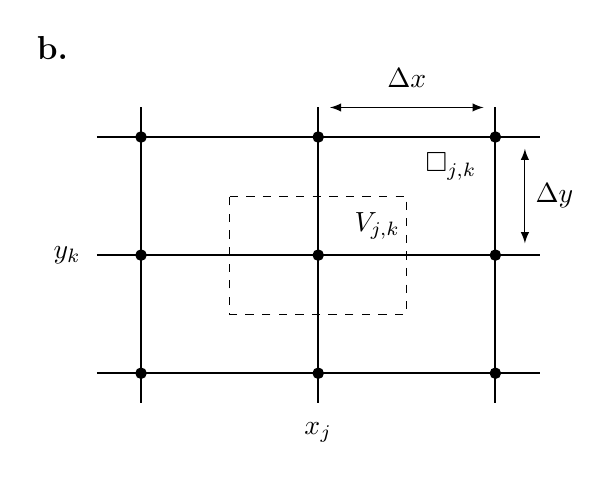
\begin{tikzpicture}[scale=0.75]
  %uncomment to see grid on which it was generated:
  %\draw[dotted,step=1.0,black,very thin] (0,0) grid (6,4);

  % strong grid around elements
  \draw[thick] (-0.75,0) -- (6.75,0);
  \draw[thick] (-0.75,2) -- (6.75,2);
  \draw[thick] (-0.75,4) -- (6.75,4);
  \draw[thick] (0,-0.5) -- (0,4.5);
  \draw[thick] (3,-0.5) -- (3,4.5);
  \draw[thick] (6,-0.5) -- (6,4.5);

  % nodes
  \filldraw (0,0) circle (2.5pt);
  \filldraw (3,0) circle (2.5pt);
  \filldraw (6,0) circle (2.5pt);
  \filldraw (0,2) circle (2.5pt);
  \filldraw (3,2) circle (2.5pt);
  \filldraw (6,2) circle (2.5pt);
  \filldraw (0,4) circle (2.5pt);
  \filldraw (3,4) circle (2.5pt);
  \filldraw (6,4) circle (2.5pt);

  % outline control volume
  \draw[dashed] (1.5,3) -- (4.5,3) -- (4.5,1) -- (1.5,1) -- cycle;

  % label element and control volume
  \draw (5.25,3.5) node {$\square_{j,k}$};
  \draw (4,2.5) node {$V_{j,k}$};

  % dimensions \Delta x, \Delta y
  \draw[latex-latex] (3.2,4.5) -- (5.8,4.5);
  \draw (4.5,5.0) node {$\Delta x$};
  \draw[latex-latex] (6.5,2.2) -- (6.5,3.8);
  \draw (7.0,3) node {$\Delta y$};

  % label center point and dims
  \draw (3,-1.0) node {$x_j$};
  \draw (-1.25,2) node {$y_k$};

  % label as "b"
  \tikzstyle{fontbf} = [font=\bf]
  \draw (-1.5,5.5) node[fontbf] {{\large b.}};
\end{tikzpicture}

\end{center}
\caption{{\large \textbf{a.}}~A structured grid as an FD grid with regular (dots) and staggered (triangles) locations.  {\large \textbf{b.}}~The same grid as an FE grid with rectangular elements (solid), nodes (dots), and dual rectangular control volumes (dashed).}
\label{fig:fdfemgrids}
\end{figure}


\section{A finite volume element interpretation} \label{sec:fveinterpretation}

The above description of the Mahaffy FD method is familiar to numerical ice sheet modelers, but deriving the same scheme from an FE or finite volume (FV) perspective \cite{LeVeque}, as we do now, is new.  Our re-interpretation uses the same structured grid, but the regular grid points $(x_j,y_k)$ are now nodes (degrees of freedom) for a continuous space of trial functions.  The same nodes are also used as centered degrees of freedom for piecewise-constant test functions which are discontinuous at the FD method's staggered grid points.  The method is both of Petrov-Galerkin FE type, because the trial and test functions come from different spaces \cite{Elmanetal2005}, and a ``finite volume element'' (FVE) method \cite{EwingLinLin2002} in which exact discrete conservation follows in the standard FV understanding.

To re-derive the scheme we suppose \eqref{eq:siasteady} holds and we take a subregion $V$ of $\Omega$.  By the divergence theorem,
\begin{equation}
  - \int_{\partial V} \bq \cdot \bn\,ds = \int_V m\, dx\,dy, \label{eq:siaasconservation}
\end{equation}
where $\partial V$ denotes the boundary of $V$, $\bn$ is the outward normal unit vector, and $ds$ the length element on the closed curve $\partial V$.  This is simply the integral form of \eqref{eq:siasteady}.

An FVE method supposes that the approximation of the solution, here denoted $H^h$, where the ``$h$'' superscript is traditional for indicating FE approximations \cite{Elmanetal2005}, lies in a finite-dimensional space of continuous functions which are defined everywhere.  In fact, these functions must be sufficiently well-behaved so that the approximate flux $\bq^h$ is defined (almost) everywhere, and can be integrated along curves.  Then integral equation \eqref{eq:siaasconservation} is required to hold for a finite set of volumes $V$, which together tile $\Omega$, and this generates a finite system of nonlinear (algebraic) equations which can be solved by Newton's method, for example (see Section \ref{sec:examples}).  This derivation of the algebraic system uses \eqref{eq:siaasconservation} as an FV method would for solving the differential equation \eqref{eq:siasteady}.  However, we could also let $g(x,y)$ be the characteristic function of $V$ (i.e.~with value one on $V$ and zero otherwise), and then multiply \eqref{eq:siasteadyfd} by $g$ and integrate and derive \eqref{eq:siaasconservation} that way, mimicking the construction of an FE method.

So consider the structured grid of $\Delta x$ by $\Delta y$ rectangles, the ``elements,'' shown in Figure \ref{fig:fdfemgrids}b.  Denote the element with lower-left corner at $(x_j,y_k)$ by $\square_{j,k}$.  These rectangles are true $Q^1$ finite elements when associated with bilinear functions, and a basis for such functions on $\square_{j,k}$ is
\begin{equation}
\chi_l(x-x_j,y-y_k), \label{eq:elementbasis}
\end{equation}
for $l=1,2,3,4$, where
\begin{align*}
\chi_1(x,y) &= \left(1-\frac{x}{\Delta x}\right) \left(1-\frac{y}{\Delta y}\right), & \chi_2(x,y) &= \frac{x}{\Delta x} \left(1-\frac{y}{\Delta y}\right), \\
\chi_3(x,y) &= \left(1-\frac{x}{\Delta x}\right) \frac{y}{\Delta y}, & \chi_4(x,y) &= \frac{x}{\Delta x} \frac{y}{\Delta y}. 
\end{align*}
If $C(\Omega)$ denotes the continuous functions on the domain, then let
\begin{equation}
S_h = \{u \in C(\Omega) \,\big|\, u \text{ is bilinear on each $\square_{j,k}$}\},
\end{equation}
the $Q^1$ finite element space \cite{Elmanetal2005}.  Functions in $S_h$ have a gradient which is defined almost everywhere, but the gradient is discontinuous along the element edges (solid lines in Figure \ref{fig:fdfemgrids}b).

Let $V_{j,k}$ be the rectangular control volume shown by dashed lines in Figure \ref{fig:fdfemgrids}b, with center at $(x_j,y_j)$, also with dimensions $\Delta x$ by $\Delta y$.  If $L^\infty(\Omega)$ denotes bounded and integrable functions on $\Omega$ \cite{Evans}, let
\begin{equation}
S_h^* = \{u \in L^\infty(\Omega) \,\big|\, u \text{ is constant on each $V_{j,k}$}\}.
\end{equation}
Functions in $S_h^*$ are discontinuous along the control volume edges (dashed lines in Figure \ref{fig:fdfemgrids}b).

Those functions which take value one at a single node and are zero at all other nodes form bases of $S_h$ and $S_h^*$, respectively.  Thus, by definition, $\psi_{j,k}(x,y)$ is the unique function in $S_h$ so that $\psi_{j,k}(x_r,y_s) = \delta_{jr} \delta_{ks}$, and $\omega_{j,k}(x,y)$ is the unique function in $S_h^*$  so that $\omega_{j,k}(x_r,y_s) = \delta_{jr} \delta_{ks}$.  See Figure \ref{fig:fembases}.  If index $j$ is in $1,\dots,N_x$ and $k$ is in $1,\dots,N_y$ then there are $N_xN_y$ distinct nodes so $\dim S_h = \dim S_h^* = N_x N_y$.  

\begin{figure}[ht]
\begin{center}
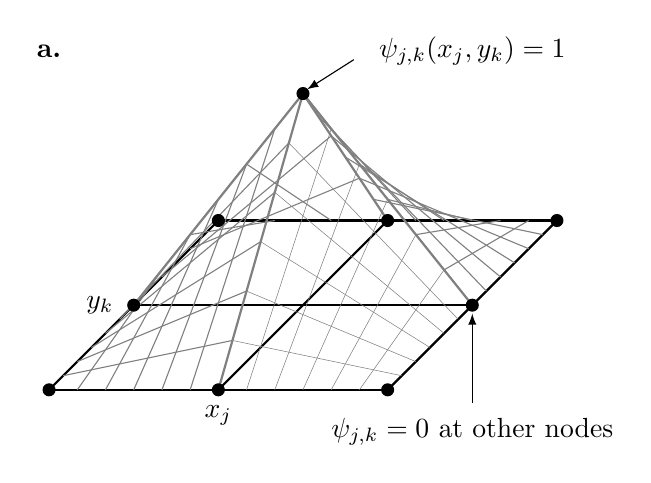
\begin{tikzpicture}[scale=8.6cm/16.0cm]
% min x = 0, max x = 12  so  width = 12 cm, but we pad
% 8.6cm is one-column width for J Glaciol
%\begin{tikzpicture}[scale=0.5]

  % strong grid around elements
  \draw[thick] (0,0) -- (8,0);
  \draw[thick] (2,2) -- (10,2);
  \draw[thick] (4,4) -- (12,4);
  \draw[thick] (0,0) -- (4,4);
  \draw[thick] (4,0) -- (8,4);
  \draw[thick] (8,0) -- (12,4);

  \def\ytop{7};

  % tent lines
  \draw[gray,thick] (6,\ytop) -- (4,0);
  \draw[gray,thick] (6,\ytop) -- (2,2);
  \draw[gray,thick] (6,\ytop) -- (10,2);
  \draw[gray,thick] (6,\ytop) -- (8,4);

  \def\dx{(10.0-6.0)/6};
  \def\dy{(2.0-\ytop)/6};
  \foreach \jj in {1,...,5}
  {
       \draw[gray,very thin] ({6+\jj*\dx},{\ytop+\jj*\dy}) -- ({4+(4/6)*\jj},0.0);
  }

  \def\dx{(4.0-6.0)/6};
  \def\dy{(0.0-\ytop)/6};
  \foreach \jj in {1,...,5}
  {
       \draw[gray,very thin] ({6+\jj*\dx},{\ytop+\jj*\dy}) -- ({10-(2/6)*\jj},{2-(2/6)*\jj});
  }

  \def\dx{(2.0-6.0)/6};
  \def\dy{(2.0-\ytop)/6};
  \foreach \jj in {1,...,5}
  {
       \draw[gray,thin] ({6+\jj*\dx},{\ytop+\jj*\dy}) -- ({4-(4/6)*\jj},0.0);
  }

  \def\dx{(4.0-6.0)/6};
  \def\dy{(0.0-\ytop)/6};
  \foreach \jj in {1,...,5}
  {
       \draw[gray,thin] ({6+\jj*\dx},{\ytop+\jj*\dy}) -- ({2-(2/6)*\jj},{2-(2/6)*\jj});
  }

  \def\dx{(10.0-6.0)/6};
  \def\dy{(2.0-\ytop)/6};
  \foreach \jj in {1,...,5}
  {
       \draw[gray,thin] ({6+\jj*\dx},{\ytop+\jj*\dy}) -- ({8+(4/6)*\jj},4.0);
  }

  \def\dx{(8.0-6.0)/6};
  \def\dy{(4.0-\ytop)/6};
  \foreach \jj in {1,...,5}
  {
       \draw[gray,thin] ({6+\jj*\dx},{\ytop+\jj*\dy}) -- ({10+(2/6)*\jj},{2+(2/6)*\jj});
  }

  \def\dx{(2.0-6.0)/3};
  \def\dy{(2.0-\ytop)/3};
  \foreach \jj in {1,...,2}  % reduce clutter
  {
       \draw[gray,thin] ({6+\jj*\dx},{\ytop+\jj*\dy}) -- ({8-(4/3)*\jj},4.0);
  }

  \def\dx{(8.0-6.0)/3};
  \def\dy{(4.0-\ytop)/3};
  \foreach \jj in {1,...,2}
  {
       \draw[gray,thin] ({6+\jj*\dx},{\ytop+\jj*\dy}) -- ({2+(2/3)*\jj},{2+(2/3)*\jj});
  }

  % nodes in base plane
  \filldraw (0,0) circle (4pt);
  \filldraw (4,0) circle (4pt);
  \filldraw (8,0) circle (4pt);
  \filldraw (2,2) circle (4pt);
  %\filldraw (6,2) circle (4pt);   % (x_j,y_k) is at (6,2)
  \filldraw (10,2) circle (4pt);
  \filldraw (4,4) circle (4pt);
  \filldraw (8,4) circle (4pt);
  \filldraw (12,4) circle (4pt);

  % node at tent top
  \filldraw (6,\ytop) circle (4pt);

  % annotate
  \draw (10,\ytop+1.0) node {$\psi_{j,k}(x_j,y_k)=1$};
  \draw[-latex] (7.2,\ytop+0.8) -- (6.1,\ytop+0.1);
  \draw (10,-1.0) node {$\psi_{j,k}=0$ at other nodes};
  \draw[-latex] (10,-0.3) -- (10,1.8);

  % label center point
  \draw (4,-0.6) node {$x_j$};
  \draw (1.2,2) node {$y_k$};

  % label as "a"
  \tikzstyle{fontbf} = [font=\bf]
  \draw (0,8) node[fontbf] {a.};

\end{tikzpicture}
 \quad 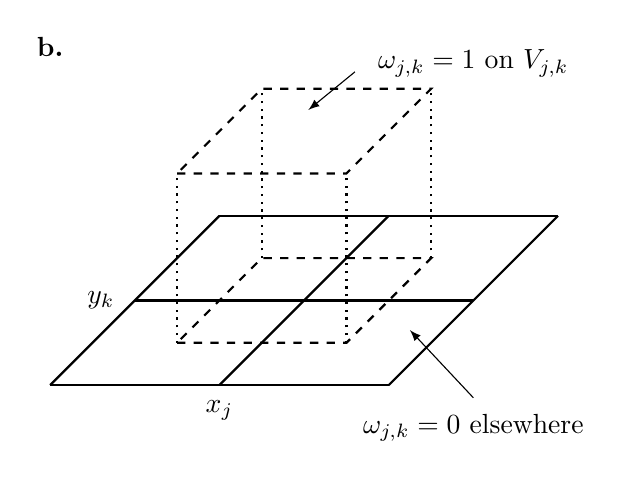
\begin{tikzpicture}[scale=8.6cm/16.0cm]
% min x = 0, max x = 12  so  width = 12 cm, but we pad
% 8.6cm is one-column width for J Glaciol
%\begin{tikzpicture}[scale=0.5]

  % strong grid around elements
  \draw[thick] (0,0) -- (8,0);
  \draw[thick] (2,2) -- (10,2);
  \draw[thick] (4,4) -- (12,4);
  \draw[thick] (0,0) -- (4,4);
  \draw[thick] (4,0) -- (8,4);
  \draw[thick] (8,0) -- (12,4);

  % dashed grid around control volume in base plane
  \draw[thick] (0,0) -- (8,0);

  % label element and control volume
  \def\lift{4};
  \draw[dashed, thick] (3,1) -- (7,1) -- (9,3) -- (5,3) -- cycle;
  \draw[dashed, thick] (3,1+\lift) -- (7,1+\lift) -- (9,3+\lift) -- (5,3+\lift) -- cycle;
  \draw[dotted, thick] (3,1) -- (3,1+\lift);
  \draw[dotted, thick] (7,1) -- (7,1+\lift);
  \draw[dotted, thick] (9,3) -- (9,3+\lift);
  \draw[dotted, thick] (5,3) -- (5,3+\lift);

  % annotate
  \draw (10,\lift+3.6) node {$\omega_{j,k}=1$ on $V_{j,k}$};
  \draw[-latex] (7.2,\lift+3.4) -- (6.1,\lift+2.5);
  \draw (10,-1.0) node {$\omega_{j,k}=0$ elsewhere};
  \draw[-latex] (10,-0.3) -- (8.5,1.3);

  % label center point
  \draw (4,-0.6) node {$x_j$};
  \draw (1.2,2) node {$y_k$};

  % label as "b"
  \tikzstyle{fontbf} = [font=\bf]
  \draw (0,8) node[fontbf] {b.};

\end{tikzpicture}

\end{center}
\caption{{\large \textbf{a.}}~A continuous ``hat'' basis function $\psi_{j,k}(x,y)$ in the $Q^1$ trial space $S_h$.  {\large \textbf{b.}}~A discontinuous, piecewise-constant basis function $\omega_{j,k}(x,y)$ in the test space $S_h^*$.}
\label{fig:fembases}
\end{figure}

We seek an approximate solution $H^h$ from $S_h$.  Let $b^h$ be the piecewise-bilinear interpolant of the bed elevation $b$, thus also in $S_h$, and let $s^h=H^h+b^h$.  We denote by $\bq^h$ the flux computed from formula \eqref{eq:siaflux} using $H^h$ and $b^h$, so that $\bq^h$ is well-defined on the interior of each element.  We require \eqref{eq:siaasconservation} to hold for this $\bq^h$ and all volumes $V_{j,k}$.  (Equivalently, we multiply \eqref{eq:siasteady} by any $\omega_{j,k}$ from the basis for $S_h^*$, and integrate, and require these equations to hold.)  However, we use midpoint quadrature on the right-hand integral in \eqref{eq:siaasconservation}.  Thus we seek $H^h$ in $S_h$ satisfying
\begin{equation}
  - \int_{\partial V_{j,k}} \bq^h \cdot \bn\,ds = m_{j,k}\, \Delta x \Delta y, \label{eq:siafve}
\end{equation}
for all $j,k$.  This equation gives a finite algebraic system once we choose a quadrature rule on the left.  Equation \eqref{eq:siafve} is a typical FV interpretation of equation \eqref{eq:siasteady}, but the FE character remains because $\bq^h$ is defined almost everywhere on $\Omega$, as $H^h$ and $s^h$ are from $S_h$.

We decompose the integral in \eqref{eq:siafve} into the four edges which form $\partial V_{j,k}$.  Let
\begin{equation}
x_j^\pm = x_j \pm \dxtwo, \qquad y_k^\pm = y_k \pm \dytwo, \label{eq:definexypm}
\end{equation}
and denote components $\bq^h = \ip{q^x}{q^y}$, so that
\begin{equation}
  \int_{\partial V_{j,k}} \bq^h \cdot \bn\,ds = \int_{y_k^-}^{y_k^+} q^x(x_j^+,y)\,dy + \int_{x_j^-}^{x_j^+} q^y(x,y_k^+)\,dx - \int_{y_k^-}^{y_k^+} q^x(x_j^-,y)\,dy - \int_{x_j^-}^{x_j^+} q^y(x,y_k^-)\,dx. \label{eq:fluxintdecomp}
\end{equation}
Note $\bq^h$ is a well-defined, bounded function, and continuous on each element $\square_{j,k}$, but it is discontinuous across element boundaries.  For example, in the first integral on the right in \eqref{eq:fluxintdecomp} the integrand $f(y) = q^x(x_j^+,y)$ is piecewise-continuous on the interval of integration $y_k^- \le y \le y_k^+$, but it has a jump discontinuity at the midpoint $y=y_k$ because, though $\grad s^h = \ip{s^h_x}{s^h_y}$ is linear on each element, $s^h_y$ is discontinuous at $y=y_k$.

The Mahaffy scheme computes each integral in \eqref{eq:fluxintdecomp} by the midpoint method, but using the value of the discontinuous component of the surface gradient \emph{computed by averaging across its jump discontinuity}.  Thus Mahaffy does not use a true quadrature, because the integrand $\bq^h\cdot \bn$ does not have a value at the quadrature (mid-) point, but a value is re-constructed.

To turn this idea into formulas, observe that the thickness $H^h$ and the $x$-derivative $s^h_x$ have continuous values between the elements $\square_{j,k}$ and $\square_{j,k-1}$.  Indeed, the components of the surface gradient on the element $\square_{j,k}$ have the formulas
	\begin{comment}
	COMMENT OUT: here is the surface elevation on $\square_{j,k}$
	\begin{align*}
	s^h(x,y) &= s_{j,k} \left(1-\tfrac{x-x_j}{\Delta x}\right) \left(1-\tfrac{y-y_k}{\Delta y}\right)
	    + s_{j+1,k} \left(\tfrac{x-x_j}{\Delta x}\right) \left(1-\tfrac{y-y_k}{\Delta y}\right) \\
	         &\qquad + s_{j,k+1} \left(1-\tfrac{x-x_j}{\Delta x}\right) \left(\tfrac{y-y_k}{\Delta y}\right)
	    + s_{j+1,k+1} \left(\tfrac{x-x_j}{\Delta x}\right) \left(\tfrac{y-y_k}{\Delta y}\right)
	\end{align*}
	\end{comment}
\begin{align}
s^h_x(x,y) &= \frac{s_{j+1,k}-s_{j,k}}{\Delta x} \left(1-\frac{y-y_k}{\Delta y}\right) + \frac{s_{j+1,k+1}-s_{j,k+1}}{\Delta x} \left(\frac{y-y_k}{\Delta y}\right), \label{eq:grads} \\
s^h_y(x,y) &= \frac{s_{j,k+1}-s_{j,k}}{\Delta y} \left(1-\frac{x-x_j}{\Delta x}\right) + \frac{s_{j+1,k+1}-s_{j+1,k}}{\Delta y} \left(\frac{x-x_j}{\Delta x}\right), \notag
\end{align}
and the same functions on $\square_{j,k-1}$ can be calculated by shifting the index $k\to k-1$.  Thus $s^h_x(x,y)$ is continuous on the interval of integration in the first integral in \eqref{eq:fluxintdecomp}, and at the midpoint it has value
\begin{equation}
s^h_x(x_j^+,y_k) = \frac{s_{j+1,k}-s_{j,k}}{\Delta x}. \label{eq:femsxstag}
\end{equation}
Similarly, writing-out $H^h(x,y)$ on each element, using the element basis \eqref{eq:elementbasis}, and evaluating at the midpoint in the first integral in \eqref{eq:fluxintdecomp} gives
\begin{equation}
H^h(x_j^+,y_k) = \frac{H_{j,k}+H_{j+1,k}}{2}, \label{eq:femHstag}
\end{equation}

However, the $y$-derivative has different values above (i.e.~on $\square_{j,k}$) and below (on $\square_{j,k-1}$) the element boundary at $y = y_k$; the limits are:
\begin{align}
s^h_y(x_j^+,y_k+0) = \frac{s_{j,k+1}-s_{j,k} + s_{j+1,k+1}-s_{j+1,k}}{2\Delta y}, \\
s^h_y(x_j^+,y_k-0) = \frac{s_{j,k}-s_{j,k-1} + s_{j+1,k}-s_{j+1,k-1}}{2\Delta y}. \notag
\end{align}
The average of these values is thus not a value of $s_y^h$, but a good re-construction thereof:
\begin{equation}
\widehat{s^h_y}(x_j^+,y_k) = \frac{s_{j,k+1} + s_{j+1,k+1} - s_{j,k-1} - s_{j+1,k-1}}{4\Delta y}. \label{eq:femsystagcrime}
\end{equation}
The hat in \eqref{eq:femsystagcrime} indicates that it is \emph{not} a result of evaluating $s^h_y(x,y)$, but formula \eqref{eq:femsystagcrime} is exactly the estimate of $\partial s/\partial y$ which appears in FD formula \eqref{eq:mahaffyWalphax}.

In our FVE interpretation, we see that the Mahaffy scheme uses \eqref{eq:femsxstag}, \eqref{eq:femHstag}, and \eqref{eq:femsystagcrime} in the midpoint rule:
\begin{equation}
\int_{y_k^-}^{y_k^+} q^x(x_j^+,y)\,dy \approx - \Gamma H^h(x_j^+,y_k)^{n+2} \left(s^h_x(x_j^+,y_k)^2 + \widehat{s^h_y}(x_j^+,y_k)^2\right)^{(n-1)/2} s^h_x(x_j^+,y_k)\,\Delta y. \label{eq:femmahaffyfirstint}
\end{equation}
Mahaffy thus approximates each integral on the right in \eqref{eq:fluxintdecomp} by a smart quadrature ``crime'' (compare \cite{Strang1972}), averaging across discontinuities to reconstruct slopes.  Approximation \eqref{eq:femmahaffyfirstint}, and the corresponding approximations of the other integrals in \eqref{eq:fluxintdecomp}, gives the same approximations of the staggered-grid fluxes as \eqref{eq:mahaffyWqx}, \eqref{eq:mahaffyWalphax}, \eqref{eq:mahaffyWqy}, and \eqref{eq:mahaffyWalphay}.  In particular, dividing the resulting approximation of equation \eqref{eq:siafve} by the control volume area $\Delta x\,\Delta y$ gives FD equation \eqref{eq:siasteadyfd}.

\section{An improved scheme on structured and unstructured grids}  \label{sec:star}

If our goal is to convert FVE equation \eqref{eq:siafve} into an algebraic equation by a choice of quadrature along the boundary of the control volume ($\partial V_{j,k}$), it is easy to propose a straightforward improvement over the Mahaffy scheme of the previous section.  To recap the situation, because $H^h$ and $s^h$ live in the $Q^1$ space of continuous, piecewise-bilinear functions $S_h$, the numerical approximation $q^h$ from formula \eqref{eq:siaflux} is defined on the interior of each element.  However, because the gradient $\grad s^h$ is discontinuous across the element boundaries, also $\bq^h$ is discontinuous across element boundaries.

Because of the discontinuity of the integrand on the element boundary, we break each interval of integration on the right-hand side of \eqref{eq:fluxintdecomp} into two parts, so that we are integrating smooth functions.  For example, we break the first integral on the right-hand side of \eqref{eq:fluxintdecomp} at $y=y_k$.  Then we use the midpoint rule, which is the optimal one-point rule for smooth functions, in each subinterval; recall notation \eqref{eq:definexypm}:
\begin{align}
  \int_{y_k^-}^{y_k^+} q^x(x_j^+,y)\,dy &= \int_{y_k^-}^{y_k} q^x(x_j^+,y)\,dy + \int_{y_k}^{y_k^+} q^x(x_j^+,y)\,dy \label{eq:starbreakfirst} \\
      &\approx \frac{\Delta y}{2} \left(q^x(x_j^+,y_k-\tfrac{\Delta y}{4}) + q^x(x_j^+,y_k+\tfrac{\Delta y}{4})\right). \notag
\end{align}
The values $q^x(x_j^+,y_k\pm\tfrac{\Delta y}{4})$ are straightforwardly-evaluated by computing $q^x(x,y)$ on the appropriate element.  Given that we index so that element $\square_{j,k}$ has lower-left corner $(x_j,y_k)$, however, note that $(x_j^+,y_k+\tfrac{\Delta y}{4})$ is a point in element $\square_{j,k}$ while $(x_j^+,y_k-\tfrac{\Delta y}{4})$ is a point in element $\square_{j,k-1}$.  Similar formulas apply to the other three integrals on the right-hand side of \eqref{eq:fluxintdecomp}.

We call this method the ``\Mstar'' method.  Figure \ref{fig:mahaffystar} shows all eight quadrature points needed to compute the full integral over $\partial V_{j,k}$ in \eqref{eq:siafve}.  Clearly the method requires evaluating $\bq^h(x,y)$ at four locations in each element.  In the sense that the Mahaffy method itself (section \ref{sec:fveinterpretation}) requires evaluating the flux at the midpoint of every side of every element, it also requires evaluating the flux at four locations in each element.  However, the total number of flux-evaluations per node is two times larger for \Mstar than for Mahaffy.  The stencils for the two methods are the same in the sense that in both methods equation \eqref{eq:siafve} uses the nine nodal values of $H^h$ and $b^h$ (solid dots in Figure \ref{fig:mahaffystar}).

\begin{figure}[ht]
\begin{center}
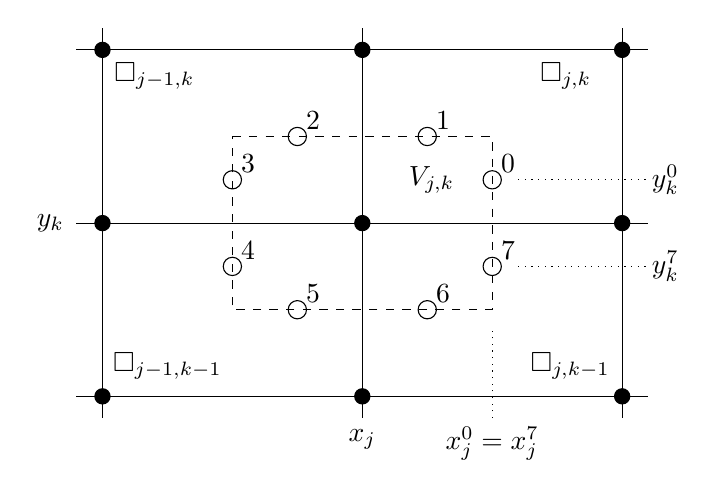
\begin{tikzpicture}[scale=1.1]
  %uncomment to see grid on which it was generated:
  %\draw[dotted,step=1.0,black,very thin] (0,0) grid (6,4);

  % strong grid around elements
  \draw (-0.3,0) -- (6.3,0);
  \draw (-0.3,2) -- (6.3,2);
  \draw (-0.3,4) -- (6.3,4);
  \draw (0,-0.25) -- (0,4.25);
  \draw (3,-0.25) -- (3,4.25);
  \draw (6,-0.25) -- (6,4.25);

  % nodes
  \filldraw (0,0) circle (2.5pt);
  \filldraw (3,0) circle (2.5pt);
  \filldraw (6,0) circle (2.5pt);
  \filldraw (0,2) circle (2.5pt);
  \filldraw (3,2) circle (2.5pt);
  \filldraw (6,2) circle (2.5pt);
  \filldraw (0,4) circle (2.5pt);
  \filldraw (3,4) circle (2.5pt);
  \filldraw (6,4) circle (2.5pt);

  % outline control volume
  \draw[dashed] (1.5,3) -- (4.5,3) -- (4.5,1) -- (1.5,1) -- cycle;

  % mark quadrature points

  \draw (4.5,2.5) circle (3.0pt) node[shift={(0.2,0.2)}] {0};
  \draw (3.75,3)  circle (3.0pt) node[shift={(0.2,0.2)}] {1};
  \draw (2.25,3)  circle (3.0pt) node[shift={(0.2,0.2)}] {2};
  \draw (1.5,2.5) circle (3.0pt) node[shift={(0.2,0.2)}] {3};
  \draw (1.5,1.5) circle (3.0pt) node[shift={(0.2,0.2)}] {4};
  \draw (2.25,1)  circle (3.0pt) node[shift={(0.2,0.2)}] {5};
  \draw (3.75,1)  circle (3.0pt) node[shift={(0.2,0.2)}] {6};
  \draw (4.5,1.5) circle (3.0pt) node[shift={(0.2,0.2)}] {7};

  % label elements and control volume
  \draw (3.8,2.5) node {$V_{j,k}$};
  \draw (5.35,3.7) node {$\square_{j,k}$};
  \draw (5.4,0.35) node {$\square_{j,k-1}$};
  \draw (0.6,3.7) node {$\square_{j-1,k}$};
  \draw (0.75,0.35) node {$\square_{j-1,k-1}$};

  % label center point
  \draw (3,-0.5) node {$x_j$};
  \draw (-0.6,2) node {$y_k$};

  % indicate coordinates of quadrature points
  \draw[dotted] (4.5,-0.25) -- (4.5, 0.8);
  \draw (4.5,-0.55) node {$x_j^0=x_j^7$};
  \draw[dotted] (4.8,2.5) -- (6.3, 2.5);
  \draw (6.5,2.5) node {$y_k^0$};
  \draw[dotted] (4.8,1.5) -- (6.3, 1.5);
  \draw (6.5,1.5) node {$y_k^7$};

\end{tikzpicture}

\end{center}
\caption{To compute the integral in equation \eqref{eq:siafve} the \Mstar method evaluates the $Q^1$ approximation of the flux $\bq^h(x,y)$ at eight locations (circles) along $\partial V_{j,k}$.}
\label{fig:mahaffystar}
\end{figure}

Indeed, eight half-edges make up $\partial V_{j,k}$, with each half-edge entirely inside an element.  Along each half-edge the $Q^1$ approximation $\bq^h$ is smooth.  Thus one could propose improved-quadrature methods, beyond \Mstar, which replace the midpoint rule by the 2-point Gauss-Legendre quadrature (thus 2 flux evaluations per half-edge, and 16 evaluations along $\partial V_{j,k}$), Simpson quadrature (3 and 24 evaluations), or other quadrature methods.  Such methods have not been tested.  Also, the $Q^1$ elements considered in this paper could be replaced by higher-order $Q^2$ elements, and so on.  However, the largest numerical errors when solving the SIA occur near the free boundary, namely at the ice sheet margin \cite{Bueleretal2005}.  At such locations the exact solution $H$ has low regularity (compare \cite{JouvetBueler2012}), and any FE method of any order suffers in the sense that the exact free boundary may pass through an element.  Because $\bq^h$ represents a smooth approximation on the element to a merely-continuous (and not smooth) exact flux $\bq$, on such free boundary elements, higher-order quadratures will probably not give much advantage.  The \Mstar method represents a measurable improvement over the Mahaffy method (see the next section) primarily because the quadrature method in \Mstar uses true evaluations of the flux approximation $\bq^h$.

FIXME: the same \Mstar idea can be extended to dual Delaunay/Voronoi meshes (e.g.~the meshes from \cite{EgholmNielsen2010,Ringleretal2013}) using $P^1$ elements on the Delaunay triangulation, and doing quadrature on the Voronoi-cell edges by splitting these edges where the element (i.e.~triangle) boundaries cross (perpendicularly) the Voronoi-cell edges.  This improves on the \cite{EgholmNielsen2010} method by exploiting an underlying $P^1$ element approximation to approximate the flux, instead of using the moving least squares method.


\section{Computed examples} \label{sec:examples}

FIXME: code \texttt{petsc/mahaffy.c} implements \Mstar and Mahaffy methods; verification relative to steady part of Test D from \cite{Bueleretal2005}, i.e.~``Bueler profile'' from \cite{vanderVeen2013}; at low res we see \Mstar is more accurate at points along margin; at high res \Mstar is slightly better for convergence

FIXME: add whole Greenland model; compute \Mstar SIA solution with present-day climate in one step on fairly high res (2km?)


\section{Conclusion} \label{sec:conclusion}

FIXME: The first idea in the paper is that a FVE interpretation is compatible with the original Mahaffy FD scheme.  The second idea is that the flux approximation is discontinuous along element edges, so, in evaluating the quadrature along the boundary of the control volume, there is either a doubling of the range over which derivatives are evaluated (Mahaffy) or a doubling of the number of quadrature points (\Mstar).  The new \Mstar method is slightly more accurate, especially at coarse resolution, and easier to understand and implement in a $Q^1$ FE world.  The computed examples using this method are novel, except for \cite{JouvetBueler2012}, by going directly to steady state from zero ice.

%         References
\bibliography{../paper/lc}
\bibliographystyle{siam}


\begin{comment}
Here is what the MPAS Land-Ice User's Manual version 3.0 says:

\begin{quote}
\small
Velocities and fluxes are calculated on the midpoint of Voronoi cell edges.  The normal component of surface slope is calculated on cell edges using surface elevation at adjacent cell centers.  The tangential component of surface slope is calculated on cell edges using surface elevation at adjacent vertices. The surface elevation at vertices is calculated from the values at adjacent cell centers using barycentric interpolation. Ice thickness on edges is calculated as the average of the adjacent cell center values (2nd-order approximation).
\end{quote}

Looking at this, and the code, I don't think they think of it as Petrov-Galerkin
\end{comment}


\end{document}
